% !TeX document-id = {d42653b9-9ea4-48c2-860b-3d6e6e9d8ab0}
% !TeX TXS-program:compile = txs:///pdflatex/[--shell-escape]
\documentclass[12pt]{article} % For LaTeX2e
%\usepackage{neurips_2021}
\usepackage[colorlinks, citecolor={blue}]{hyperref}
\usepackage{url}
\usepackage{amsfonts,amscd,amssymb}
\usepackage{amsthm,amsmath,natbib}
\usepackage{algorithm,algorithmicx,algpseudocode}
\usepackage{bm}
\usepackage{bbm} %bb font numbers
\usepackage[table]{xcolor}
\usepackage{verbatim}
\usepackage{graphicx}
\usepackage{setspace}
\usepackage{natbib}
\usepackage[margin=1in]{geometry}
\usepackage{enumitem}
%\usepackage[nolists]{endfloat}
\usepackage{listings}
\usepackage[textsize=tiny]{todonotes}
\usepackage{tikz}
\usetikzlibrary{shapes.misc}
\usepackage{etoolbox}
\usepackage{appendix}
\usepackage[format=plain,
labelfont={it},
textfont=it]{caption}
\usepackage{subcaption}
\usepackage{wrapfig}
\usepackage{xr}
\usepackage{booktabs}
\usepackage{multirow}
\usepackage{authblk}
\usepackage{mathbbol}
\usepackage{thmtools}



\usetikzlibrary{matrix}
\usetikzlibrary{backgrounds}
\usetikzlibrary{calc}
\usetikzlibrary{arrows,shapes}
\usetikzlibrary{decorations}
\usetikzlibrary{decorations.pathmorphing}
\usetikzlibrary{fit}
\usetikzlibrary{decorations.pathreplacing}
\usetikzlibrary{shapes.misc}
\usetikzlibrary{shapes.geometric}

\newtoggle{quickdraw}
%\toggletrue{quickdraw} % Uncomment this to render more quickly (non-random)


\definecolor{lightgrey}{rgb}{0.9,0.9,0.9}
\definecolor{darkgreen}{rgb}{0,0.3,0}
%\definecolor{darkred}{rgb}{0.3,0,0}

\definecolorset{rgb}{}{}{darkred,0.8,0,0;darkgreen,0,0.5,0;darkblue,0,0,0.5}

%\doublespacing

\newtheorem{thm}{Theorem}
\newtheorem{lemma}{Lemma}
\newtheorem{prop}{Proposition}
\newtheorem{cor}{Corollary}
\newtheorem{remark}{Remark}
\newtheorem{example}{Example}
\newtheorem{mydef}{Definition}
\newtheorem*{assumption}{Assumption}
\newtheorem{clm}{Claim}

\newcommand{\argmax}{\operatornamewithlimits{arg\,max}}
\newcommand{\argmin}{\operatornamewithlimits{arg\,min}}
\newcommand*{\fplus}{\genfrac{}{}{0pt}{}{}{+}}
\newcommand*{\fdots}{\genfrac{}{}{0pt}{}{}{\cdots}}
\newcommand{\mb}{\mathbf}
\newcommand{\mc}{\mathcal}
\newcommand{\dx}{\mbox{d}}

\renewcommand{\vec}[1]{\mathbf{#1}}
\newcommand{\numTaxa}{N}
\newcommand{\numTraits}{D}
\newcommand{\numDatasets}{M}
%\newcommand{\numLatent}{D}
\newcommand{\taxonIndex}{i}
\newcommand{\traitIndex}{j}
\newcommand{\traitData}{\vec{Y}}
\newcommand{\traitDatum}{y}
\newcommand{\datasetIndex}{m}
\newcommand{\exemplar}{\text{e}}

\newcommand{\sequences}{\vec{S}}
\newcommand{\latentData}{\vec{X}}
\newcommand{\latentdata}{\vec{x}}
\newcommand{\latentDatum}{x}
\newcommand{\phylogeneticParameters}{\boldsymbol{\phi}}
\newcommand{\phylogeny}{{\cal G}}
\newcommand{\tree}{\phylogeny}
%\newcommand{\otherParameters}{\boldsymbol{\
\newcommand{\transpose}{^{t}}

\newcommand{\distanceMatrix}{\mathbf{Y}}
\newcommand{\distance}{y}
\newcommand{\summant}{r}



\newcommand{\cdensity}[2]{\ensuremath{p(#1 \,|\,#2)}}
\newcommand{\density}[1]{\ensuremath{p(#1 )}}

\newcommand{\treeNode}{\nu}

\newcommand{\traitVariance}{\mathbf{\Sigma}}
\newcommand{\nodeIndex}{c}

%\newcommand{\parent}[1]{\mbox{\tiny pa}(#1)}
\newcommand{\parentBig}[1]{\mbox{pa}(#1)}

\newcommand{\sibling}[1]{\mbox{\tiny sib}(#1)}
\newcommand{\siblingBig}[1]{\mbox{sib}(#1)}

\newcommand{\rootMean}{\boldsymbol{\mu}_0}
\newcommand{\rootVarianceScalar}{\tau_0}
\newcommand{\unsequencedVarianceScalar}{\tau_{\exemplar}}
\newcommand{\treeVariance}{\vec{V}_{\tree}}
\newcommand{\hatTreeVariance}{\hat{\vec{V}}_{\tree}}
\newcommand{\mdsSD}{\sigma}
\newcommand{\mdsVariance}{\mdsSD^2}
\newcommand{\residual}{\hat{\traitDatum}}
\newcommand{\modelDistance}{\delta}
\newcommand{\cdf}{\phi}
\newcommand{\normalCDF}[1]{\Phi \left( #1 \right)}

\newcommand{\order}[1]{{\cal O}\hspace{-0.2em}\left( #1 \right)}

\newcommand{\rootNode}{\nu^{\datasetIndex}_{2 \numTaxa_{\datasetIndex} -1 }}
\newcommand{\pathLength}[1]{d(F, #1 )}
\newcommand{\pathLengthNew}[2]{
d_{F}
(
{#1}, {#2}
)
}
\newcommand{\J}{\vec{J}}
\newcommand{\pprime}{^{\prime}}
\newcommand{\otherIndex}{i \pprime}
\def\kronecker{\raisebox{1pt}{\ensuremath{\:\otimes\:}}}

\definecolor{trevorblue}{rgb}{0.330, 0.484, 0.828}
\definecolor{trevoryellow}{rgb}{0.829, 0.680, 0.306}


\allowdisplaybreaks

%\makeatletter
%\def\title@font{\Huge}
%\let\ltx@maketitle\@maketitle
%\def\@maketitle{\bgroup%
%	\let\ltx@title\@title%
%	\def\@title{\resizebox{\textwidth}{!}{%
%			\mbox{\title@font\ltx@title}%
%	}}%
%	\ltx@maketitle%
%	\egroup}
%\makeatother


\title{Matrix exponential derivative}


%\date{}



\author{Andrew J.~Holbrook}

 
\affil{UCLA Biostatistics}





\renewcommand\Authands{ and }


\graphicspath{{figures/}}

\begin{document}


\maketitle




\begin{abstract}

I investigate the accuracy of the first-order approximation to the directional derivative of the matrix exponential of CTMC generator matrices.


\end{abstract}



\section{Introduction}\label{sec:intro}

%\newcommand{\x}{\mathbf{x}}
%\renewcommand{\v}{\mathbf{v}}

%\newcommand{\TTTheta}{\boldsymbol{\Theta}}
%\newcommand{\tr}{\mbox{tr}}
%\newcommand{\X}{\mathbf{X}}
%\renewcommand{\u}{\mathbf{u}}
\newcommand{\QQ}{\mathbf{Q}}
\newcommand{\DD}{\mathbf{D}}
\newcommand{\MM}{\mathbf{M}}
\newcommand{\JJ}{\mathbf{J}}
\newcommand{\II}{\mathbf{I}}
\newcommand{\RR}{\mathbf{R}}
%\newcommand{\haar}{\mathcal{H}}
%\newcommand{\orthog}{\mathcal{O}}
%\newcommand{\SSigma}{\boldsymbol{\Sigma}}
\newcommand{\Zero}{\boldsymbol{0}}
\newcommand{\ttheta}{\boldsymbol{\theta}}


Let $\QQ=[q_{ij}]$ be the rate matrix for an $S$-dimensional continuous time Markov chain, where $q_{ij}>0$ for $i\neq j$, and $q_{ii} = -\sum_{j\neq i} q_{ij}$.  We are interested in quickly approximating the directional derivative of the matrix exponential
\begin{align*}
	\exp(t\QQ) = \sum_{k=0}^\infty \frac{t^k\QQ^k}{k!}
\end{align*}
for arbitrary $t>0$ using the formula \citep{najfeld1995derivatives}
\begin{align}\label{eq:deriv}
	\nabla_{\MM} \exp(t\QQ)  =  \exp(t\QQ)  \sum_{k=0}^\infty \frac{t^{k+1}}{(k+1)!} \{\MM,\QQ^k\} \, .
\end{align}
Here, $\MM$ gives the direction and $\{\MM,\QQ^k\}$ is the matrix commutator series satisfying the recursion
\begin{align*}
	\{\MM,\QQ^0\} &= \MM \, , \\ 
	\{\MM,\QQ^k\} &= [\{\MM,\QQ^{k-1}\} , \QQ]  = \{\MM,\QQ^{k-1}\} \QQ - \QQ \{\MM,\QQ^{k-1}\} \, .
\end{align*}
%In particular, we are interested in the derivative with respect to all $S^2$ $q_{ij}$, and these collectively correspond to the derivative in the direction of the matrix
%\begin{align*}
%\JJ := \begin{bmatrix}
%	1 & 1 &\cdots & 1 \\
%1&	1 &   & \\
%\vdots && \ddots& \\
%	1 & &  & 1 
%	\end{bmatrix}  \, .
%\end{align*}
%Letting $\Zero$ denote the zero matrix, the identities
%\begin{align*}
%\QQ\JJ&=\Zero \quad \mbox{and}\\
%\exp(t\QQ) \JJ &= \JJ 
%\end{align*}
%lead to fact
%\begin{align*}
% \exp(t\QQ)	\{\JJ , \QQ^1\} &=  \exp(t\QQ)	\left( \JJ  \QQ - \QQ \JJ     \right) \\
%&= \JJ \QQ \, .
%\end{align*} 
%Further, if we assume $ \exp(t\QQ)	\{\JJ , \QQ^{k}\} = \JJ\QQ^{k} $ for $k\geq0$, we have
%\begin{align*}
% \exp(t\QQ)	\{\JJ , \QQ^{k+1}\} &= \exp(t\QQ)  \left( 	\{\JJ , \QQ^{k}\} \QQ - \QQ 	\{\JJ , \QQ^{k}\} \right)  \\
% &= \JJ\QQ^{k} \QQ - \exp(t\QQ) \QQ 	\{\JJ , \QQ^{k}\} \\
% &= \JJ\QQ^{k+1}  - \QQ \exp(t\QQ)  \{\JJ , \QQ^{k}\} \\ 
% &= \JJ\QQ^{k+1} - \QQ \JJ \QQ^k \\
% &= \JJ \QQ^{k+1} \, ,
%\end{align*}
%where we use the fact that $\exp(t\QQ) \QQ = \QQ \exp(t\QQ)$. By an inductive argument, we may therefore write the following special case for $\eqref{eq:deriv}$:
%\begin{align}\label{eq:deriv2}
%	\nabla_{\JJ} \exp(t \QQ)  &=  \sum_{k=0}^\infty \frac{t^{k+1}}{(k+1)!} \JJ \QQ^k  = \JJ  \sum_{k=0}^\infty \frac{t^{k+1}}{(k+1)!}  \QQ^k \, .
%\end{align}
%This formula has an intuitive interpretation.   The derivative of the matrix power $\QQ^k$ in any direction $\MM$ is
%\begin{align}\label{eq:power}
%	\lim_{h\rightarrow 0}  \frac{(\QQ+h\MM)^k - \QQ^k }{h} = \sum_{p=1}^k  \QQ^{k-p} \MM \QQ^{p-1} \, ,
%\end{align}
%and the right-hand side reduces to $\JJ\QQ^{k-1}$ when we set $\MM=\JJ$.  Thus, Formula \eqref{eq:deriv2} naturally follows from the application of Equation \eqref{eq:power} to the individual terms within the series expansion of $\exp(t\QQ)$.
%A second expansion due to \citet{najfeld1995derivatives} achieves faster convergence:
%\begin{align}
%	\nabla_{\MM} \exp(t\QQ)  =  t\exp(t\QQ/2)  \sum_{k=0}^\infty \frac{\{\MM,(t\QQ/2)^{2k}\} }{(2k+1)!} \exp(t\QQ/2) \, .
%\end{align}
%Similar arguments to those above provide the result
%\begin{align}\label{eq:deriv3}
%	\nabla_{\JJ} \exp(t\QQ)  =  t \sum_{k=0}^\infty  \frac{t^{2k}}{2^{2k}(2k+1)!} \JJ\QQ^{2k}\exp(t\QQ/2) \, .
%\end{align}

%\subsection{First-order approximations}
%
%One may use Formula \eqref{eq:deriv2} to define the 1st-order approximation 
%\begin{align*}
%		\widetilde{\nabla}_{\JJ} \exp(t \QQ)  :=  t \JJ  
%\end{align*}
%and residual term
%\begin{align*}
%	\widetilde{\RR} := \JJ \sum_{k=1}^\infty \frac{t^{k+1}}{(k+1)!}  \QQ^k \, .
%\end{align*}
%Alternatively, one may use Formula  \eqref{eq:deriv3} to define the 1st-order approximation
%\begin{align*}
%		\widehat{\nabla}_{\JJ} \exp(t \QQ)  :=  t \JJ  \exp(t\QQ/2)
%\end{align*}
%and its respective residual
%\begin{align*}
%	\widehat{\RR} := t \sum_{k=1}^\infty  \frac{t^{2k}}{2^{2k}(2k+1)!} \JJ\QQ^{2k}\exp(t\QQ/2) \,.
%\end{align*}
%
%
%
%\section{Gradients and directional derivatives}

\newcommand{\Llambda}{\boldsymbol{\Lambda}}

%\noindent
%\citet{najfeld1995derivatives} describe the relationship between the $ij$th directional derivative $\nabla_{\JJ_{ij}} \exp(t\QQ)$ and the gradient of the $ij$th entry of $\exp(t\QQ)$ with respect to $\QQ$
%\begin{align*}
%	\frac{\partial \exp(t\QQ)_{ij}}{\partial \QQ} := \begin{bmatrix}
%	 \frac{\partial \exp(t\QQ)_{ij} }{\partial q_{11}} & \dots &  \frac{\partial \exp(t\QQ)_{ij} }{\partial q_{1S}} \\
%	 \vdots & \ddots & \\
%	  \frac{\partial \exp(t\QQ)_{ij} }{\partial q_{S1}} & &  \frac{\partial \exp(t\QQ)_{ij} }{\partial q_{SS}} 
%	\end{bmatrix} \, .
%\end{align*}
%In particular, they show the following result (Equation 145):
%\begin{align*}
%\frac{	\partial \exp(t\QQ)_{ij}}{\partial \QQ} = \nabla_{\JJ_{ij}} \exp(t\QQ^T) =\exp(t\QQ^T)  \sum_{k=0}^\infty \frac{t^{k+1}}{(k+1)!} \{\JJ_{ij},(\QQ^T)^k\}
%\end{align*}
%Now, suppose that $\theta$ is a scalar value and $\QQ$ derives from an unstructured matrix $\Llambda$ with elements $\lambda_{kl}>0$ satisfying
%\begin{align*}
%	q_{kl} = \bigg\{ \begin{matrix}
%		\lambda_{kl} \,,& k \neq l \\
%	\lambda_{kl}	-\sum_{l'=1}^S\lambda_{kl'} \, , &  k= l 
%	\end{matrix} \quad .
%\end{align*}
%Then it follows that
%\begin{align}\label{eq:together}
%	\frac{\partial \exp(t\QQ)_{ij}}{\partial \theta} &= \sum_{klmn} \frac{\partial \exp(t\QQ)_{ij}}{\partial q_{kl}} \frac{\partial q_{kl}}{\partial \lambda_{mn} } \frac{\partial \lambda_{mn}}{\partial \theta} \\  \nonumber
%	&= \sum_{klmn}  \left[ \nabla_{\JJ_{ij}} \exp(t\QQ^T) \right]_{kl} \Big(\delta_{km} \big( \delta_{kl} \left(\delta_{mn}-1\right) + \delta_{ln}\left(1-\delta_{kl}\right) \big) \Big) \frac{\partial \lambda_{mn}}{\partial \theta}  \, .
%\end{align}
%A special case of \citet{najfeld1995derivatives} (Equation 142), the identity
%\begin{align*}
%\nabla_{\JJ_{ij}} \exp(t\QQ^T) = \left( \nabla_{\JJ_{ji}} \exp(t\QQ) \right)^T 
%\end{align*}
%allows us to write \eqref{eq:together} as
%\begin{align*}
%		\frac{\partial \exp(t\QQ)_{ij}}{\partial \theta} &=  \sum_{klmn}  \left[ \left( \nabla_{\JJ_{ji}} \exp(t\QQ) \right)^T  \right]_{kl} \Big(\delta_{km} \big( \delta_{kl} \left(\delta_{mn}-1\right) + \delta_{ln}\left(1-\delta_{kl}\right) \big) \Big) \frac{\partial \lambda_{mn}}{\partial \theta} \\
%		&\approx  \sum_{klmn}  \left[ \left( t \exp(t\QQ) \JJ_{ji} \right)^T  \right]_{kl} \Big(\delta_{km} \big( \delta_{kl} \left(\delta_{mn}-1\right) + \delta_{ln}\left(1-\delta_{kl}\right) \big) \Big) \frac{\partial \lambda_{mn}}{\partial \theta} \\
%		&= \sum_{klmn}  \left[  t \JJ_{ij} \exp(t\QQ)^T \right]_{kl} \Big(\delta_{km} \big( \delta_{kl} \left(\delta_{mn}-1\right) + \delta_{ln}\left(1-\delta_{kl}\right) \big) \Big) \frac{\partial \lambda_{mn}}{\partial \theta} \, ,
%\end{align*}
%where we have made use of the first-order approximation of Formula \eqref{eq:deriv}.
%

\noindent
Let $\JJ_{ij}$ be the matrix $ij$th element equal to 1 and remaining elements equal to 0.  Then the first-order approximation to the derivative in the direction $\JJ_{ij}$ is $t \exp(t\QQ)\JJ_{ij}$.

\section{Bounding truncation error}

How good is the first order approximation $t \exp(t\QQ)\JJ_{ij}$ to the directional derivative?  In other words, we wish to know the magnitude of
\begin{align*}
err_{ij}(\QQ) =	\Vert\nabla_{\JJ_{ij}} \exp(t\QQ) - t \exp(t\QQ)\JJ_{ij} \Vert = \left\Vert \exp(t\QQ)  \sum_{k=1}^\infty \frac{t^{k+1}}{(k+1)!} \{\JJ_{ij},\QQ^k\} \right\Vert \, .
\end{align*}

\subsection{Upper bound 1}



For a submultiplicative matrix norm, we have
\begin{align*}
	\Vert \{\MM_1, \MM_2^k \}  \Vert \leq 2^k \Vert \MM_1\Vert \Vert\MM_2 \Vert ^k \, .
\end{align*}
We use this to obtain our first upper bound on $err_{ij}(\QQ)$:
\begin{align*}
	err_{ij}(\QQ) &= \left\Vert \exp(t\QQ)  \sum_{k=1}^\infty \frac{t^{k+1}}{(k+1)!} \{\JJ_{ij},\QQ^k\} \right\Vert  \\
	&\leq \Vert \exp(t\QQ) \Vert \sum_{k=1}^\infty \left\Vert \frac{t^{k+1}}{(k+1)!} \{\JJ_{ij},\QQ^k\} \right\Vert  \\
	&=  \Vert \exp(t\QQ) \Vert \sum_{k=1}^\infty \frac{t}{k+1} \frac{(2t \Vert \QQ \Vert)^k}{k!}\\
	&= \Vert \exp(t\QQ) \Vert   \frac{\exp(2t\Vert \QQ \Vert)-2t\Vert\QQ\Vert-1}{2\Vert \QQ \Vert} 
\end{align*}


\subsection{Upper bound 2}

We start with another representation of the derivative \citep{al2009computing}:
\begin{align*}
	\nabla_{\JJ_{ij}} \exp(t\QQ) = \sum_{k=1}^\infty \frac{t^k}{k!} \sum_{p=1}^k \QQ^{p-1} \JJ_{ij} \QQ^{k-p} 
\end{align*}
and the fact that
the fact that, for the Frobenius norm $\Vert \cdot \Vert_F$, we have \citep{wu2010short}
\begin{align*}
	\Vert [\MM_1,\MM_2] \Vert_F \leq \sqrt{2} \Vert \MM_1 \Vert_F \Vert \MM_2\Vert_F \, .
\end{align*}
Using these results, the truncation error may be rewritten
\begin{align*}
err_{ij}(\QQ)  &=\left\Vert - t\exp(t\QQ) \JJ_{ij}  +  \sum_{k=1}^\infty \frac{t^k}{k!} \sum_{p=1}^k \QQ^{p-1} \JJ_{ij} \QQ^{k-p}\right\Vert_F \\
&= \left\Vert \sum_{k=1}^\infty \frac{t^k}{k!} \left( \left( \sum_{p=1}^k \QQ^{p-1} \JJ_{ij} \QQ^{k-p} \right) - k \QQ^{k-1} \JJ_{ij} \right)  \right\Vert_F\\
&= \left\Vert \sum_{k=1}^\infty \frac{t^k}{k!} \sum_{p=1}^k \QQ^{p-1} \JJ_{ij} \QQ^{k-p}  -  \QQ^{k-1} \JJ_{ij} \right\Vert_F \\
&=\left\Vert  \sum_{k=1}^\infty \frac{t^k}{k!} \sum_{p=1}^{k-1} \QQ^{p-1} \JJ_{ij} \QQ^{k-p}  -  \QQ^{k-1} \JJ_{ij}\right\Vert_F \\
&=\left\Vert  \sum_{k=1}^\infty \frac{t^k}{k!} \sum_{p=1}^{k-1} \QQ^{p-1}\left( \JJ_{ij} \QQ^{k-p}  -  \QQ^{k-p} \JJ_{ij} \right)\right\Vert_F \\
&= \left\Vert  \sum_{k=1}^\infty \frac{t^k}{k!} \sum_{p=1}^{k-1} \QQ^{p-1}[\JJ_{ij}, \QQ^{k-p}] \right\Vert_F  \\
&\leq  \sum_{k=1}^\infty \frac{t^k}{k!} \sum_{p=1}^{k-1} \Vert \QQ^{p-1} \Vert_F \Vert[\JJ_{ij}, \QQ^{k-p}]\Vert_F 
\leq \sqrt{2}  \sum_{k=1}^\infty \frac{t^k}{k!} \sum_{p=1}^{k-1} \Vert \QQ^{k-1} \Vert_F  \\
&= \sqrt{2}  \sum_{k=1}^\infty \frac{t^k}{k!} (k-1) \Vert \QQ \Vert_F^{k-1} = \sqrt{2} \frac{e^{t\Vert \QQ\Vert_F}(t\Vert\QQ\Vert_F - 1) + 1}{\Vert \QQ \Vert_F} \, .
\end{align*}

\section{An approach that assumes convergence}
The above bounds appear most useful when $t$ is small.
 When $t$ is large enough that the CTMC has reached stationarity, we have 
 \begin{align*}
 	\frac{d}{dt}e^{t\QQ} =  \QQ e^{t\QQ}=e^{t\QQ} \QQ  = \Zero \, .
 \end{align*}
 If we further assume $\QQ$ is diagonalizable, i.e., $\QQ=\MM \DD \MM^{-1}$ for 
 \begin{align*}
 	\DD = \begin{Bmatrix}
 		d_1& 0 &\dots & & \\
 		0  & d_1 &0  & \dots& \\
 		\vdots &0 & \ddots & \\
 		 & \vdots& & d_{S-1} &0 \\
 		 &&&0&0
 	\end{Bmatrix} \, ,
 \end{align*}
 where $d_1,\dots,d_{S-1}<0$ are unique, then we may define a the generalized inverse $\QQ^+=\MM \DD^{+} \MM^{-1}$ of $\QQ$. Here, $\DD^+$ is the Moore-Penrose pseudoinverse obtained by inverting the non-zero elements of $\DD$.  Using this definition, it follows that

		\begin{align*}
			err_{ij}(\QQ) &=	\Vert\nabla_{\JJ_{ij}} \exp(t\QQ) - t \exp(t\QQ)\JJ_{ij} \Vert = \left\Vert \exp(t\QQ)  \sum_{k=1}^\infty \frac{t^{k+1}}{(k+1)!} \{\JJ_{ij},\QQ^k\} \right\Vert \\
		&=\left\Vert \exp(t\QQ) \JJ_{ij}  \sum_{k=1}^\infty \frac{t^{k+1}}{(k+1)!} \QQ^k \right\Vert \\
		&= \left\Vert \exp(t\QQ) \JJ_{ij} \QQ^+ \sum_{k=1}^\infty \frac{t^{k+1}}{(k+1)!} \QQ^{k+1} \right\Vert \\
		&= \left\Vert \exp(t\QQ) \JJ_{ij} \QQ^+ \left( \exp(t\QQ)-t\QQ-\II \right) \right\Vert  \, .
	\end{align*}
But $\QQ\exp(t\QQ)= \Zero$ implies $\QQ^+\exp(t\QQ)= \Zero$ because $\QQ$ and $\QQ^+$ share the same zero eigenvalue. We therefore have
\begin{align*}
err_{ij}(\QQ) &=t \left\Vert \exp(t\QQ) \JJ_{ij} \QQ^+ \left( \QQ+\II \right) \right\Vert 
\end{align*}
The matrix argument of this last term is nilpotent, so its spectral radius is 0.  Then for any $\epsilon>0$ a norm exists that is less than $\epsilon$ when applied to the matrix argument.

\subsection{Is this approach useful in high dimensions?}

This approach seems useful in higher dimensions.  In this context, the moduli of the non-zero eigenvalues appear to grow large (Figure \ref{fig:eigenvalues}).  As a result, CTMC for unstructured and high-dimensional $\QQ$ appear to reach stationarity faster.

\begin{figure}[!t]
	\centering
	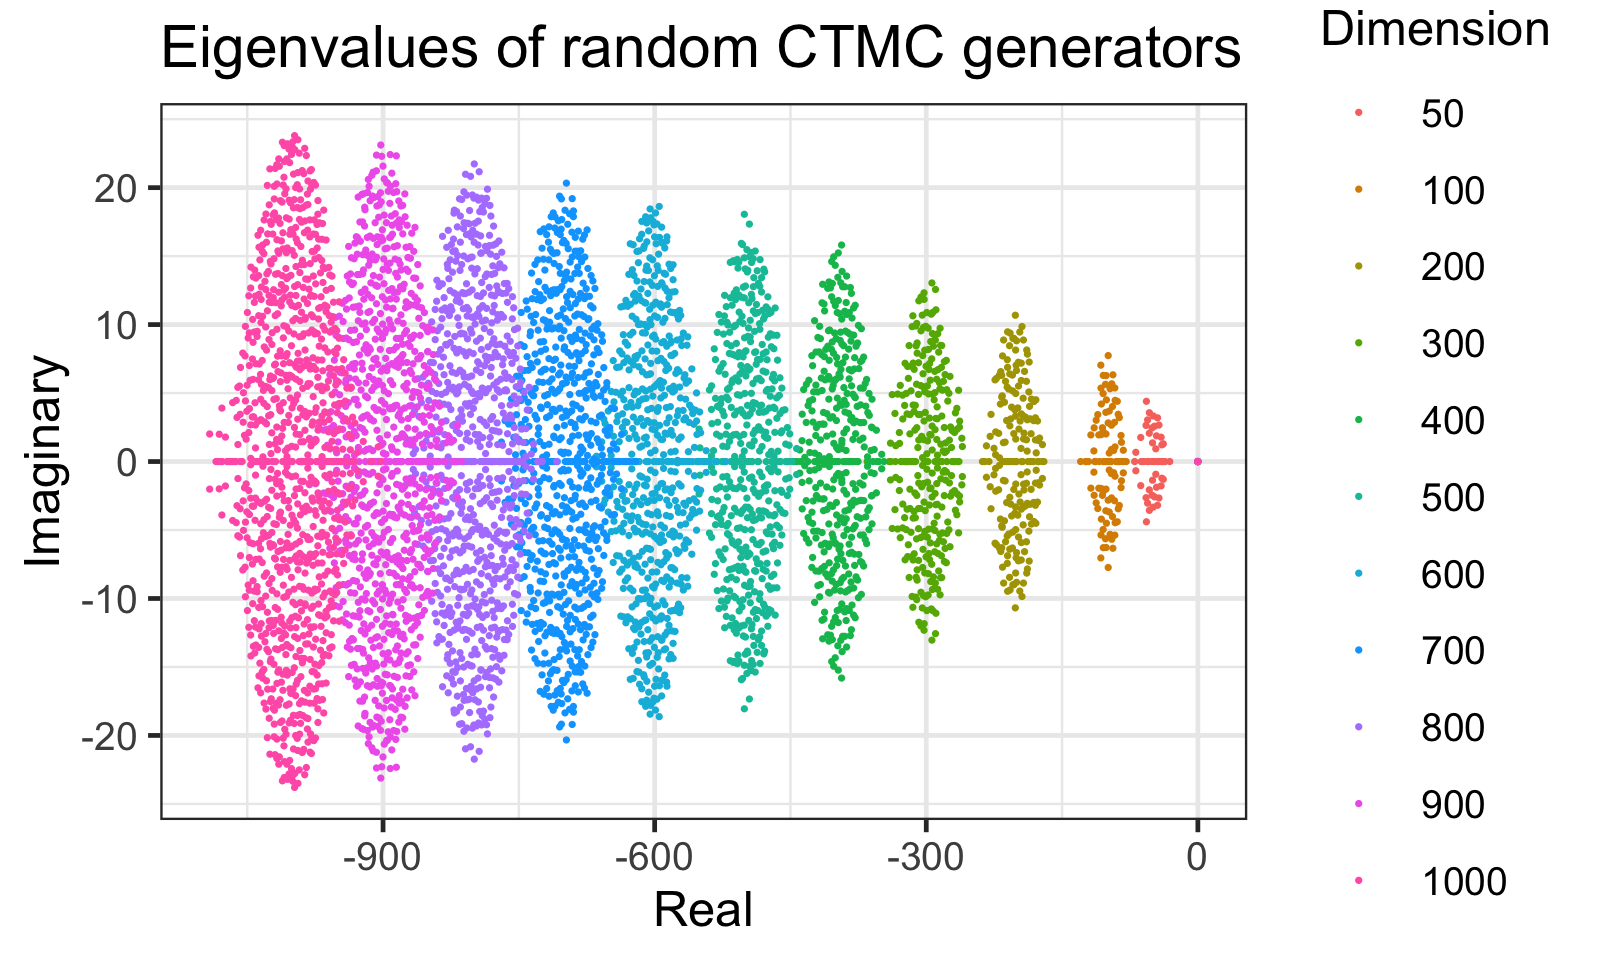
\includegraphics[width=0.9\linewidth]{eigenvaluesPlot.png}
	\caption{Eigenvalues of $\QQ$ for off-diagonal elements generated according to univariate/standard exponential distribution. Eigenvalues move farther leftward for larger dimensions.  Pattern holds for other univariate distributions.}\label{fig:eigenvalues}
\end{figure}

%\section{Plugging in $\QQ^T$}
%
%We wish to evaluate
%\begin{align*}
%	\nabla_\JJ \exp(t\QQ^T) =  \exp(t\QQ^T)  \sum_{k=0}^\infty \frac{t^{k+1}}{(k+1)!} \{\JJ,(\QQ^{T})^k\} \, .
%\end{align*}
%As above, we note that for $k=1$
%\begin{align*}
%	\exp(t\QQ^T) \{ \JJ, \QQ^T\} &= \exp(t\QQ^T)  (\JJ \QQ^T - \QQ^T\JJ ) \\ 
%	&= - \exp(t\QQ^T) \QQ^T\JJ \\
%	&= - \QQ^T \exp(t\QQ^T)  \JJ =- \QQ^T \JJ \, .
%\end{align*}
%An inductive argument reveals
%\begin{align*}
%	\nabla_\JJ \exp(t\QQ^T)  =  - \sum_{k=0}^\infty \frac{t^{k+1}}{(k+1)!}( \QQ^T)^k \JJ  =  - \left( \sum_{k=0}^\infty \frac{t^{k+1}}{(k+1)!}( \QQ^T)^k \right) \JJ \, .
%\end{align*}
%
%\section{The whole thing}



\bibliographystyle{sysbio}
\bibliography{refs}

%\section{Empirical accuracy of the extra-dimensional simplicial sampler}\label{sec:qqplots}
%
%We do not prove that the extra-dimensional sampler leaves the target distribution invariant, but limited simulations suggest it might.  Figure \ref{fig:accuracy} displays quantile-quantile plots for the sampler using a simplex with 101 vertices and targeting 3D Gaussian and mixture of two Gaussian distributions.  
%
%\begin{figure}[t!]
%	\centering
%	\includegraphics[width=\linewidth]{accuracyFig.png}
%	\caption{Quantile-quantile plots for the extra-dimensional sampler using a simplex with 101 vertices targeting a 3D Gaussian and mixture of two Gaussian distributions.}\label{fig:accuracy}
%\end{figure}

%\section{Empirically optimal acceptance rates for multiple-try Metropolis}\label{sec:mtmScaling}
%
%\citet{bedard2012scaling}
%
%\begin{figure}[t!]
%	\centering
%	\includegraphics[width=0.8\linewidth]{mtmScaling.pdf}
%	\caption{Optimal acceptance rates from 20 independent MCMC runs for each dimensionality of the a standard normal target}\label{fig:accuracy}
%\end{figure}


%%%%%%%%%%%%%%%%%%%%%%%%%%%%%%%%%%%%%%%%%%%%%%%%%%%%%%%%%%%%

\end{document}
